\documentclass[a4paper,12pt,tikz,UTF8]{article}
\usepackage{amsmath}
\usepackage{amssymb}
\usepackage{graphics}
\usepackage{graphicx}
\usepackage{epstopdf}
\usepackage{inputenc}
\usepackage{geometry}
\usepackage{float}
\usepackage{epigraph}
\usepackage{pstricks}
\usepackage{tikz}
\usepackage{ifthen}
\usepackage{enumerate}
\usepackage[inline]{enumitem}
\usetikzlibrary{arrows,shapes,snakes,automata,backgrounds,petri}

\title{\bf Artipixoids!\\\large The Concept (draft)}
\author{by Andrey Zamaraev\\a5kin@github.com}

\setlength{\parindent}{0ex}
\setlength{\parskip}{1em}
\setlength\epigraphrule{0pt}
\graphicspath{ {img/} }

\begin{document}

  \maketitle

  \epigraph{
    \it 2D body, 2D brain,\\
    2D pleasure, 2D pain.
  }{--- Flatlander credo}

  \textbf{Artipixoids!} is half generative art, half artificial life project with a focus on genetic cellular automata obeying energy conservation principle. Started in the end of 2014, it has undergone several major modifications, and is still in development. But now is the right time to share basic concepts underlying all previous modifications, so others could use it to build their own wonderful worlds.

  The document is split up in two parts. In \textit{The Manifesto} we will outline the main areas of the project development, and the main goals per each area. In \textit{The Core} section, we will give the formal definitions to the features we would like to see in the core of our future framework. 

  \newpage
  \tableofcontents

  \newpage
  \section{The Manifesto}

  \subsection{Artistic}
  \label{subsec:manifest-artistic}

    \begin{enumerate}
      \item We are going to generate the beautiful objects of abstract digital arts, even at the cost of computational resources.
      \item The objects of arts are: static images, videos, sounds, 3D models, etc.
      \item We will consider the object as Artipixoid if and only if:
        \begin{enumerate}
          \item \label{itm:valid-artipixoid} the object is generated by CA fulfilling all the definitions from section~\ref{sec:the-core} (The Core);
          \item the object's generative algorithm is not using anything but CA states as input;
          \item the object's generative algorithm is not based on the objects of arts, other than Artipixoids (eg. deep art based on Van Gogh paintings or photos doesn't count, but deep art based on other Artipixoids is OK).
        \end{enumerate}
      \item Artipixoids that has no artistic value are bad and a subject to genocide.
      \item Yet, if at least one person found them beautiful, we let them live.
    \end{enumerate}

  \subsection{Scientific}
  \label{subsec:manifest-scientific}
  \begin{enumerate}

    \item We are going to make experiments to test the hypothesis that a life can self-organize in artificial (digital) environment from a random initial state.

    \item \textbf{\textit{The properties of life}}, as we see it, are following.
      \begin{enumerate}
        \item \textit{Integrity:} every lifeform should be distinct from its local environment, and should preserve its individuality during the lifespan.
        \item \textit{Sustainability:} a lifeform should be able to self-repair in case of damage, and to maintain the physical manifestation (body) for a long enough period of time.
        \item \textit{Reproductivity:} a lifeform should be able to replicate, creating new individuals with small enough differences to consider them inexact copy.
        \item \textit{Novelty:} new lifeforms should arise out of the old ones, and they should act more effectively than the old ones. 
        \item \textit{Diversity:} there should be enough different lifeforms to put them in groups called 'species'.
        \item \textit{Complementarity:} different species should learn to live in symbiosis and help each other to survive and improve, forming stable ecosystems.
        \item \textit{Adaptability:} species should learn to evolve in a way they are constantly adapting to aggressive environmental changes.
      \end{enumerate}

    \item \textbf{\textit{The properties of artificial environment}}, as we see it, are following.
      \begin{enumerate}

        \item \textit{Discreteness:} the space and time of our environment should be discrete. So, space should consist of indivisible quanta, and their updates should occur in separate timesteps synchronously. In addition, any parameter of spatial quanta should take integer values only. This requirements will allow us to run the simulation of our environment on modern digital computational systems.
        \item \textit{Determinancy:} a global state of the environment at the timestep $t$ should lead to one and only one global state at the timestep $t + 1$. This will give us ensurance of the exactly same outcome, every time we run a particular experiment with the same initial state.
        \item \textit{Locality:} each quantum should have the same number and the same topology of its neighbors, and quantum's state should be updated using nothing more than the states of its neighbors and its own state. This will allow us to exploit the massively parallel computations, thus greatly speeding up the simulation.
        \item \label{itm:isolation} \textit{Isolation:} the environment as a whole should behave like an isolated thermodynamic system. So, each quantum should have an energy level, and sum of all quanta's energy levels should be a constant value. Energy conservation will make us sure, that none of our experiments will lead neither to the extinction nor to the explosion of 'matter'.
        \item \textit{Isotropy:} all possible reflections of quantum's neighborhood at the timestep $t$ should lead to the same new quantum's state at timestep $t + 1$. This will allow energy to spread in all possible directions uniformly. 
        \item \textit{Polymorhism:} each quantum should have a microprogram, influencing its local update rules to some degree. A microprogram in return could also be changed according to update rules. This will allow us to add genetic informational component to the quantum level. We believe, this component is the key for the emergence of self-organized matter effects at the higher (macro) levels.
        \item \textit{Stochasticity:} optionally, some pseudorandom component would influence local updates too. For that, each quanta should have its own PRNG with long enough period. This will allow energy to spread in chaotic clouds, rather than in direct lines.
        \item \textit{Mutability:} optionally, a quantum's microprogram would randomly mutate over time. This will result in wider genetic search for better microprograms, and also may prevent the whole environment from being conquested by a single genome.
        \item \textit{Magnetism:} optionally, quanta would have the tendency to 'attract' each other with some sort of force (gravitational, electromagnetic, or any other). We believe, magnetism is another key aspect behind the phenomenon of life as we know it.
      \end{enumerate}

    \item \textbf{\textit{Random initial state}}, could be obtained using following known patterns.
      \begin{enumerate}
        \item \textit{'Primordial Soup':} each and every quantum initially has an equally small amount of energy, other parameters are random. This is a good test for the ability of energy to self-organize in clusters from the completely uniform distribution. The bigger clusters are, the better. Fractal clusters are even better.
        \item \textit{'Big Bang':} a small area of space is initialized with a high amount of energy and random parameters per each quantum. Outside the area, quanta has either zero or minimum possible amount of energy. This is a good test for the ability of energy to spread in empty space. We could also detect the fastest types of energy using this pattern. 
        \item \textit{'Super Cluster':} same as Big Bang, but several areas with a bit lower energies are randomly initialized. The positions of areas are random across the space. This is a good test for gravitational effects, and also for collisions of different energy beams, produced in micro-bangs.
      \end{enumerate}

    \item To obtain the better results, we reserve the rights to intervene the natural process of evolution. This will ruin the idea of self-emergence, but still may prove the possibility of artificial life in our environment.\\\\
          \textbf{\textit{The presumable methods of intervention}} are following.
      \begin{enumerate}
        \item \textit{Genetic selection:} during the simulation, we are collecting the most interesting and promising areas of space, then combine them all in a single initial state and repeat the process recursively while novel phenomena of interest are showing up.
        \item \textit{Directed mutation (a.k.a. 'Hand of Fate')}: during the simulation, we are occasionaly pointing our finger to a small area of interest, and all quanta in this area are randomly changing parameters, excluding energy level. Then, evolution continues. 
        \item \textit{Pre-designed components:} we are designing patterns of matter manually quantum by quantum, then using them either as a parts of more complex designs or to impact on 'raw' matter in some way.
      \end{enumerate}

  \end{enumerate}

  \subsection{Divine}

  \begin{enumerate}
    \item We, as young goddesses and gods, are willing to create worlds with one click of our fingers. Actually, it doesn't have to be a click, a tap of one finger is even better.
    \item After the tap, we are willing to say the Word, which contains the essence of the future world.
    \item Then, the world begins to bloom, and it blooms the same every time we say the same Word.
    \item Some of us will just meditate on the beauty of their worlds, wandering around and changing the views.
    \item Others will actively play demiurges using scientific wizardry from previous section, or even more powerful stuff.
    \item And some will get bored and destroy the creation with a single tap of the finger. Thus, letting its habitants live in some parallel universe, free of divine will and happy.
  \end{enumerate}

  \subsection{Social}

  \begin{enumerate}
    \item We are going to build the community over those who interested in any of previously mentioned ideas.
    \item For that, we need a framework, implementing basic CA engine described below, along with a set of modular tools to easily build engine modifications.
    \item Then, we will be able to exchange new modifications in a form of compact modules.
    \item We will also be able to exchange new modular tools and extend our framework with them for future re-using.
    \item Finally, for each modification, we will be able to make a collection of the experiment files with initial state and hyperparameters included, and run them in uniform interactive environment on massively parallel hardware like GPU clusters.
  \end{enumerate}

  \subsection{Alien}

  Nothing there yet. This section is reserved just to fit the law of fives. 

  \newpage

  \section{The Core}
  \label{sec:the-core}

  There is a special subclass of cellular automata that allows us to implement all the properties of environment described in section~\ref{subsec:manifest-scientific}. We call it \textit{Buffered State Cellular Automata} (BSCA). In this section, we will give the formal definition of all BSCA features, to be integrated in the core of our future framework.

  \subsection{Grid and neighborhood topologies}

    As in any CA, grid in BSCA is $D$-dimensional lattice of cells, each having $N$ neighbors. $(D, N) \in [1 .. \infty)$.

    The cells are stored in a sequence of length $M$:
    \begin{equation}
      \label{eq:cells}
      C = \langle c_0, ..., c_{M - 1} \rangle, \quad M \in {[1 .. \infty)},
    \end{equation}
    where elements are nested sequences with uniform structure called \textit{cell state}. See the exact definition of the cell state in Eq.~17 below. We may refer to $C$ as to a \textit{board state} later.

    The cartesian coordinates of the cell with index $i$ could be obtained as 
    \begin{equation}
      [ x_0, ..., x_{D - 1} ] = \chi(i), \quad i \in {[0 .. M)},
    \end{equation}
    where $\chi$ is \textit{lattice topology function}. 

    Let also define a sequence of all cells' coordinates as 
    \begin{equation}
      X = \langle \chi(0), ..., \chi(M - 1) \rangle.
    \end{equation}
    We may refer to $X$ as to just a \textit{board} later.

    The cartesian coordinates of cell's $j$-th neighbor could be obtained as
    \begin{equation}
      [ x_0, ..., x_{D - 1} ] = \nu(X_i, j), \quad i \in {[0 .. M)}, \quad j \in {[1 .. N]},
    \end{equation}
    where $\nu$ is \textit{neighborhood topology function}. 

    Thus, we will assume the whole grid topology is homogeneous if and only if the following equation holds for each value of $j$:
    \begin{equation}
      X_i - \nu(X_i, j) = d_j, \quad \forall i \in {[0 .. M)}, j \in [1 .. N],
    \end{equation}
    where $d_j$ is a constant vector for each $j$. So, the vector difference between the positions of cell and its $j$-th neighbor should be a constant for each cell in a grid.

  \subsection {Border Effects}

    A \textit{border cell} is a cell, having at least one of its neighbours off the board $X$. If $A_i$ is a set of all $i$-th cell's neighbors, that are inside $X$:
    \begin{equation}
      A_i = \{ C_i \mid \nu(X_i, j) \in X, j \in [1 .. N] \}, \quad i \in {[0 .. M)},
    \end{equation}
    then the following inequality holds for all border cells:
    \begin{equation}
      | A_i | \neq N, \quad i \in [0 .. M).
    \end{equation}

    In order to correctly process all cells, including border ones, we have to define a conditional function $\eta$ for neighbors obtainment. Let call it a \textit{neighbour function}:
    \begin{equation}
      \eta(i, j) = 
      \begin{cases}
        C_{\chi^{-1}(\nu(X_i, j))} & \quad \text{if } \nu(X_i, j) \in X,\\  
        \beta(\nu(X_i, j)) & \quad \text{if } \nu(X_i, j) \notin X,
      \end{cases}
    \end{equation}
    where $\beta$ is a \textit{border function} returning a state for a hypothetic cells outside $X$, and $\chi^{-1}$ is a reverse lattice topology function, satisfying the following equation:
    \begin{equation}
      \chi^{-1}(\chi(i)) = i.
    \end{equation}

    Border function $\beta$ could take a variety of forms. It could just be a constant pre-defined state (static borders). Or wrap borders into higher dimensional manifold topology, like torus, M{\"o}ebius strip or Klein bottle. It could even yield a random state each time.

    In case of wrapping, the border function will take a form of
    \begin{equation}
      \label{eq:border-function-wrapping}
      \beta(x) = C_{\beta^*(x)}, \quad \beta^*(x) \in {[0 .. M)},
    \end{equation}
    where $\beta^*$ is a \textit{wrap function}, mapping off-board coordinates to other cells on the board, and on-board coordinates strictly to the cells with those coordinates:
    \begin{equation}
      \beta^*(x) = 
      \begin{cases}
        \chi^{-1}(x) & \quad \text{if } x \in X,\\
        i \in {[0 .. M)} & \quad \text{if } x \notin X.
      \end{cases}
    \end{equation}

    We will assume that the whole grid neighborhood is homogeneous if and only if the border function takes a form as in Eq.~\ref{eq:border-function-wrapping}, and the following condition holds:
    \begin{equation}
      \label{eq:neighborhood-homogeneity}
      C_i \in \{ \eta(i', j) \mid j \in {[1 .. N]} \}, \quad i' \in \{ \beta^*(\nu(X_i, j)) \mid j \in {[1 .. N]} \}, \quad i \in {[0 .. M)},
    \end{equation}
    so, each cell should be present in a set of neighbours for all of its neighbours.

    Be warned, any border function that breaks the neighborhood homogeneity, may also break an energy conservation, unless the buffered interactions with off-board cells are explicitly restricted in update rules. See Section~\ref{subsec:energy-conservation} for more details.

  \subsection{Single Cell Design}

    Let recursively define a \textit{parameter} as either an integer or a sequence of parameters. Then, the infinite set $P$ of all possible parameters is
    \begin{align}
      \begin{split}
        P_0 &= \mathbb{Z},\\
        P_{n + 1} &= \bigcup_{i=1}^\infty{P_n^i,}
      \end{split}
    \end{align}
    thus we can say that $p$ is a \textit{parameter} if and only if $p \in P$.

    Let also define a recursive function $\varphi$, that will replace all integers with zeros in a parameter:
    \begin{equation}
      \varphi(p) = 
      \begin{cases}
        0 \quad & \text{if } p \in \mathbb{Z},\\
        \langle \varphi(p_0), ..., \varphi(p_{|p|-1}) \rangle \quad & \text{if } p \notin \mathbb{Z}.
      \end{cases}
    \end{equation}

    We will call $\varphi$ \textit{parameter topology function}, and will assume two parameters $p_1$ and $p_2$ have the same topology if and only if the following equation holds:
    \begin{equation}
      \varphi(p_1) = \varphi(p_2).
    \end{equation}

    The \textit{generic state} then is a parameter with the constant topology within a particular BSCA. Let define $S_s$ as a set of all possible generic states:
    \begin{equation}
      S_s = \{ s \mid s \in P, \varphi(s) = p_c \},
    \end{equation}
    where $p_c$ is a constant topology value.

    \begin{figure}[h]
      \centering
      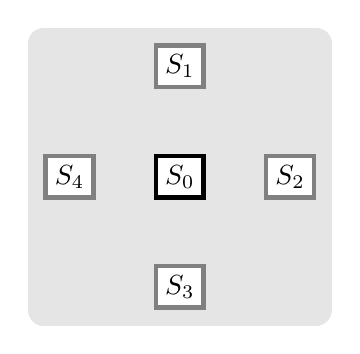
\begin{tikzpicture}[node distance=1.4cm]
        \tikzstyle{main}=[rectangle, ultra thick, draw=black!100, fill=white!100, minimum size=4mm]
        \tikzstyle{buffer}=[rectangle, ultra thick, draw=black!50, fill=white!100, minimum size=4mm]
        \begin{scope}
          \node [main] (s0) {$S_0$};
          \node [buffer] (s1) [above of=s0] {$S_1$};
          \node [buffer] (s2) [right of=s0] {$S_2$};
          \node [buffer] (s3) [below of=s0] {$S_3$};
          \node [buffer] (s4) [left of=s0] {$S_4$};
        \end{scope}
        \begin{pgfonlayer}{background}
          \filldraw [line width=4mm, join=round, black!10]
          (s1.north  -| s2.east)  rectangle (s3.south  -| s4.west);
        \end{pgfonlayer}
      \end{tikzpicture}
      \caption{Single cell design in BSCA.}
      \label{fig:cell-design}
    \end{figure}

    The \textit{cell state} $c$ (see Eq.~\ref{eq:cells}) is a sequence of $N + 1$ generic states:
    \begin{equation}
      \label{eq:cell-state}
      c = \langle S_0, ..., S_N \rangle, \quad S_i \in S_s \forall i \in {[0 .. N]},
    \end{equation}
    where $S_0$ is the \textit{main state}, and $S_1$, ..., $S_N$ are the \textit{buffered states}, one per each neighbor. At the Fig.~\ref{fig:cell-design}, you can see a cell design for 2-dimensional BSCA with Von Neumann neighborhood. Buffered neighbor states is the cruicial aspect of BSCA, it is the basic feature allowing us to implement lossless models with energy exchanges and genome crossbreeding across all neighbor cells. See more on this topic in the sections below.

    Let also define two more sets for future use:
    \begin{align}
      S_c &= S_s^{N + 1},\\
      S_b &= S_c^M,
    \end{align}
    where $S_c$ is a set of all possible cell states, and $S_b$ is a set of all possible board states.

  \subsection{Time and Updates}

    The \textit{universe} is a board state evolving in discrete timesteps. Let define the universe $U$ as a potentially infinite recurrent sequence:
    \begin{align}
      \begin{split}
        U_0 &= C_s,\\
        U_{t + 1} &= \omega(U_t),
      \end{split}
    \end{align}
    where $C_s$ is an \textit{initial board state} (also called \textit{seed}), $t$ is a timestep number and $\omega: S_b \to S_b$ is an \textit{update function}.

    In BSCA, the evolution at a single timestep is going in two phases: \textit{emit phase} and \textit{absorb phase}, so update function will take a form of
    \begin{equation}
      \omega(u) = \alpha(\varepsilon(u)),
    \end{equation}
    where $\alpha$ is \textit{absorb function} and $\varepsilon$ is \textit{emit function}. Let describe how both of them works in the next sections.

  \subsection{Emit Phase}

    \begin{figure}[H]
      \centering
      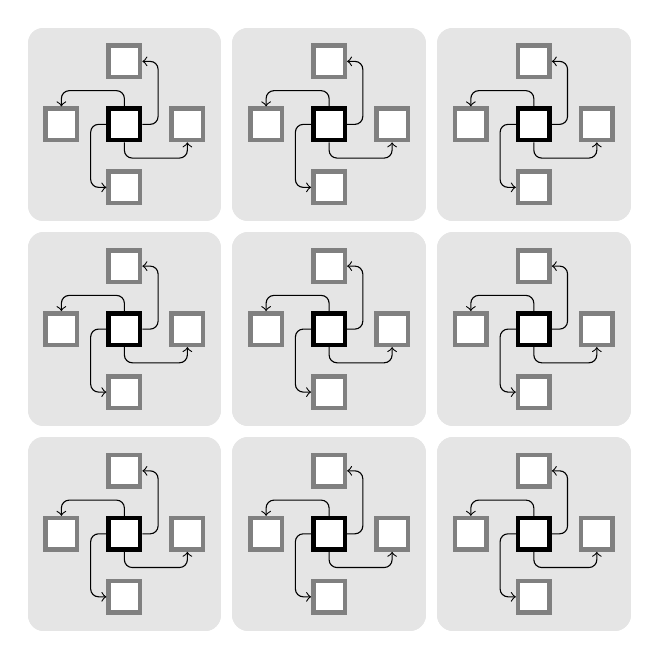
\begin{tikzpicture}[node distance=8mm]
        \tikzstyle{main}=[rectangle, ultra thick, draw=black!100, fill=white!100, minimum size=4mm]
        \tikzstyle{buffer}=[rectangle, ultra thick, draw=black!50, fill=white!100, minimum size=4mm]
        \pgfmathtruncatemacro{\gridsize}{2};
        \pgfmathtruncatemacro{\cellsize}{26};
        \foreach \x in {0, ..., \gridsize}
          \foreach \y in {0, ..., \gridsize}
          {
            \pgfmathtruncatemacro{\xs}{\x * \cellsize};
            \pgfmathtruncatemacro{\ys}{\y * \cellsize};
            \begin{scope}[xshift=\xs mm,yshift=\ys mm]
              \node [main] (s0\x\y) {};
              \node [buffer] (s1\x\y) [above of=s0\x\y] {};
              \node [buffer] (s2\x\y) [right of=s0\x\y] {};
              \node [buffer] (s3\x\y) [below of=s0\x\y] {};
              \node [buffer] (s4\x\y) [left of=s0\x\y] {};
            \end{scope}
            \begin{pgfonlayer}{background}
              \filldraw [line width=4mm, join=round, black!10]
              (s1\x\y.north  -| s2\x\y.east)  rectangle (s3\x\y.south  -| s4\x\y.west);
            \end{pgfonlayer}
          }
        \foreach \x in {0, ..., \gridsize}
          \foreach \y in {0, ..., \gridsize}
          {
            \pgfmathtruncatemacro{\xs}{\x * \cellsize};
            \pgfmathtruncatemacro{\ys}{\y * \cellsize};
            \begin{scope}[xshift=\xs mm,yshift=\ys mm,rounded corners=1mm]
              \draw[->] (s0\x\y.east) -- +(.2,0) |- (s1\x\y.east);
              \draw[->] (s0\x\y.south) -- +(0,-.2) -| (s2\x\y.south);
              \draw[->] (s0\x\y.west) -- +(-.2,0) |- (s3\x\y.west);
              \draw[->] (s0\x\y.north) -- +(0,.2) -| (s4\x\y.north);
            \end{scope}
            \begin{pgfonlayer}{background}
              \filldraw [line width=4mm, join=round, black!10]
              (s1\x\y.north  -| s2\x\y.east)  rectangle (s3\x\y.south  -| s4\x\y.west);
            \end{pgfonlayer}
          }
      \end{tikzpicture}
      \caption{Emit Phase in BSCA.}
      \label{fig:emit-phase}
    \end{figure}

    The process of emit is like sending the messages from a cell to its neighbors. Each cell performs it as follows.
    \begin{enumerate}
      \item 
        The cell is taking a sequence of all its neighbors' main states, as well as its own main state:
        \begin{equation}
          \label{eq:neighbors-main-sequence}
          \eta_e(C, i) = \langle \gamma({C_i}, 0), \gamma(\eta(i, 1), 0), ..., \gamma(\eta(i, N), 0) \rangle,
        \end{equation}
        where $i$ is the cell's index and $\gamma$ is a function for obtaining an item from the sequence:
        \begin{equation}
          \label{eq:item-obtaining}
          \gamma(s, i) = s_i.
        \end{equation}
      \item
        The cell is modifying its buffers and main state as a result of \textit{decision function} $\sigma: S_c \to S_c$:
        \begin{equation}
          \label{eq:decision-function}
          C_i := \sigma(\eta_e(C, i)),
        \end{equation}
        where $i$ is the cell's index and $C$ is a board state at the current timestep $t$: $C = U_t$. The decision function $\sigma$ could be as complex as you need: from naive copy of main state to sophisticated microprogram execution.
      \item
        At the end of emit phase, each buffer should contain a generic state intended for a specific neighbor.
    \end{enumerate}

    The whole emit function $\varepsilon: S_b \to S_b$ thus takes a form of
    \begin{equation}
      \varepsilon(C) = \langle \sigma(\eta_e(C, 0)), ..., \sigma(\eta_e(C, M - 1)) \rangle,
    \end{equation}

    Fig.~\ref{fig:emit-phase} shows the emit phase for 2-dimensional BSCA with Von Neumann neighborhood. The arrows are indicating the updates. So, at this phase, the main states are read-only, and the buffers are write-only within every given cell, which makes the process ``thread safe''.

  \subsection{Absorb Phase}

    \begin{figure}[H]
      \centering
      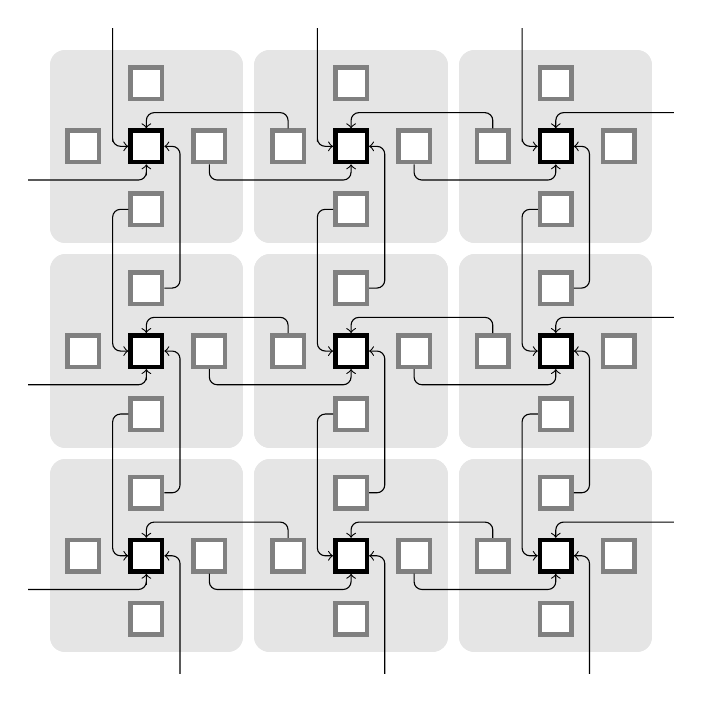
\begin{tikzpicture}[node distance=8mm]
        \tikzstyle{main}=[rectangle, ultra thick, draw=black!100, fill=white!100, minimum size=4mm]
        \tikzstyle{buffer}=[rectangle, ultra thick, draw=black!50, fill=white!100, minimum size=4mm]
        \pgfmathtruncatemacro{\gridsize}{2};
        \pgfmathtruncatemacro{\cellsize}{26};
        \foreach \x in {0, ..., \gridsize}
          \foreach \y in {0, ..., \gridsize}
          {
            \pgfmathtruncatemacro{\xs}{\x * \cellsize};
            \pgfmathtruncatemacro{\ys}{\y * \cellsize};
            \begin{scope}[xshift=\xs mm,yshift=\ys mm]
              \node [main] (s0\x\y) {};
              \node [buffer] (s1\x\y) [above of=s0\x\y] {};
              \node [buffer] (s2\x\y) [right of=s0\x\y] {};
              \node [buffer] (s3\x\y) [below of=s0\x\y] {};
              \node [buffer] (s4\x\y) [left of=s0\x\y] {};
            \end{scope}
            \begin{pgfonlayer}{background}
              \filldraw [line width=4mm, join=round, black!10]
              (s1\x\y.north  -| s2\x\y.east)  rectangle (s3\x\y.south  -| s4\x\y.west);
            \end{pgfonlayer}
          }
        \foreach \x in {0, ..., \gridsize}
          \foreach \y in {0, ..., \gridsize}
          {
            \pgfmathtruncatemacro{\xs}{\x * \cellsize};
            \pgfmathtruncatemacro{\ys}{\y * \cellsize};
            \pgfmathtruncatemacro{\xp}{\x + 1};
            \pgfmathtruncatemacro{\xm}{\x - 1};
            \pgfmathtruncatemacro{\yp}{\y + 1};
            \pgfmathtruncatemacro{\ym}{\y - 1};
            \begin{scope}[xshift=\xs mm,yshift=\ys mm,rounded corners=1mm]
              \ifthenelse{\x < \gridsize}{
                \draw[->] (s4\xp\y.north) -- +(0,.2) -| (s0\x\y.north);
              }{
                \draw[<-] (s0\x\y.north) -| +(0,.2) -- +(1.5,.2);
              }
              \ifthenelse{\ym > -1}{
                \draw[->] (s1\x\ym.east) -- +(.2,0) |- (s0\x\y.east);
              }{
                \draw[<-] (s0\x\y.east) -- +(.2,0) |- +(.2,-1.5);
              }
              \ifthenelse{\xm > -1}{
                \draw[->] (s2\xm\y.south) -- +(0,-.2) -| (s0\x\y.south);
              }{
                \draw[<-] (s0\x\y.south) |- +(0,-.2) -- +(-1.5,-.2);
              }
              \ifthenelse{\y < \gridsize + 2}{
                \draw[->] (s3\x\yp.west) -- +(-.2,0) |- (s0\x\y.west);
              }{
                \draw[<-] (s0\x\y.west) -| +(-.2,0) -- +(-.2,1.5);
              }       
            \end{scope}
            \begin{pgfonlayer}{background}
              \filldraw [line width=4mm, join=round, black!10]
              (s1\x\y.north  -| s2\x\y.east)  rectangle (s3\x\y.south  -| s4\x\y.west);
            \end{pgfonlayer}
          }
      \end{tikzpicture}
      \caption{Absorb Phase in BSCA.}
      \label{fig:absorb-phase}
    \end{figure}

    At the absorb phase, each cell is receiving buffered states as ``messages'' from its neighbors, then evolving. It goes as follows.
    \begin{enumerate}
      \item 
        From each neighbor, the cell is taking a buffered state intended for itself, and making a sequence from these states, along with its own main state:
        \begin{equation}
          \label{eq:neighbors-main-sequence}
          \eta_a(C, i) = \langle \gamma({C_i}, 0), \gamma(\eta(i, 1), \iota^{-1}(i)), ..., \gamma(\eta(i, N), \iota^{-1}(i)) \rangle,
        \end{equation}
        where $i$ is the cell's index, $\gamma$ is a function from Eq.~\ref{eq:item-obtaining}, and $\iota^{-1}: \mathbb{Z} \to \mathbb{Z}$ is the function for reverse neighbor index obtaining, for which the following equation holds:
        \begin{equation}
          \eta(i, j) = \eta(\chi^{-1}(\nu(X_i, j)), \iota^{-1}(j)).
        \end{equation}
      \item
        The cell is modifying its own main state as a result of \textit{blend function} $\psi: S_c \to S_c$:
        \begin{equation}
          \label{eq:blend-function}
          C_i := \psi(\eta_a(C, i)),
        \end{equation}
        where $i$ is the cell's index and $C$ is a board state at the current timestep $t$: $C = U_t$. The blend function $\psi$ is generally performing a combination of incoming buffer states. It could be a sum or mean value or some genome crossover etc. Although, no one can keep you from inventing more exotic blend functions.
      \item
        At the end of absorb phase, each cell's main state is evolved and a subject to the observation, you can record it, use in visualization and so on.
    \end{enumerate}

    The whole absorb function $\alpha: S_b \to S_b$ thus takes a form of
    \begin{equation}
      \alpha(C) = \langle \psi(\eta_a(C, 0)), ..., \psi(\eta_a(C, M - 1)) \rangle,
    \end{equation}

    Fig.~\ref{fig:absorb-phase} shows the absorb phase for 2-dimensional BSCA with Von Neumann neighborhood. The arrows are indicating the updates. So, at this phase, the buffered states are read-only, and the main states are write-only within every given cell, which in combination with emit phase, gives us the ability to safely run the whole process on massively parallel architectures.

  \subsection{Energy conservation}
    \label{subsec:energy-conservation}
    Using the design from previous sections, it is very easy to define a model that will behave like an isolated thermodynamic system (see Item~\ref{itm:isolation} from Section~\ref{subsec:manifest-scientific}). If $E: S_s \to \mathbb{Z}$ is a function for extracting the energy component from the generic state, then we can say the system will obey the energy conservation principle if the following equations holds:
    \begin{equation}
      \label{eq:emit-conservation}
      \sum_{i=0}^{N}{E(c_i)} = \sum_{i=0}^{N}{E(\gamma(\sigma(c), i))}, \quad \forall c \in S_c,
    \end{equation}
    \begin{equation}
      \sum_{i=0}^{N}{E(c_i)} = \sum_{i=0}^{N}{E(\gamma(\psi(c), i))}, \quad \forall c \in S_c.
    \end{equation}
    Thus, the summed energy should stay the same for the argument and the result of either decision or blend function.

    The broken neighborhood homogeneity (see Eq.~\ref{eq:neighborhood-homogeneity}) could easily be a threat for energy conservation. For example, in a case of static borders the energy may leak over the edge of the board. To prevent this, we must restrict buffered interactions with the off-board cells: at the emit phase, all the buffers pointing over the edge should be set to a state of zero energy, and Eq.~\ref{eq:emit-conservation} should still be held.

    Please also note, energy conservation is the mandatory criteria for ``genuine'' Artipixoids (see Item~\ref{itm:valid-artipixoid} from Section~\ref{subsec:manifest-artistic}).

  \subsection{Genetic Microprograms}

    As we stated in The Manifesto, informational component is the key aspect to the phenomenon of life as we know it. Without information, the energy would just be a dull clouds of dust wandering randomly in space and time. But, as we all can see, the matter is organizing in the complex self-replicating patterns, and this is happening at each level of existense: from galaxies to atoms. We believe, this principle of self-organization is scaling fractally from the very bottom level of indivisible Planck scale quanta, each behaving like a machine executing a genetic microprogram.

    Since the cell is the smallest unit in our artificial environment, it's a good candidate for microprogram execution. For that, it must have several pre-defined parameters:
    \begin{itemize}
      \item an integer parameter $p_p$ to hold an execution pointer;
      \item an integer parameter $p_m$ to hold a set of microinstructions (program memory), $L_m$ bits in total, $L_c$ bits per instruction, $L_m, L_c \in {[1 .. \infty)}$;
      \item a sequence of integer parameters to hold some values (registers): $p_r = \langle p_{r_0}, p_{r_1}, ... \rangle$ 
    \end{itemize}

    Then, at the emit phase the cell acts as follows:
    \begin{enumerate}
      \item Incrementing execution pointer, and returning it to the beginning as needed:
        \begin{equation}
          p_p = (p_p + 1) \text{ mod } (L_m / L_c).
        \end{equation}
      \item Obtaining a microinstruction at the position of execution pointer:
        \begin{equation}
          p_i = (p_m \text{ lsh } (p_p * L_c)) \text{ and } (2^{L_c} - 1).
        \end{equation}
      \item Modifying its own state as shown in Eq.~\ref{eq:decision-function}, but the decision function is gotten from the pre-defined sequence of functions, one function per each microinstruction:
        \begin{equation}
          \sigma \Leftrightarrow \sigma_{p_i}.
        \end{equation}
        Thus, the decision function is depending on the current microinstruction.
    \end{enumerate}

    We may consider a microprogram's memory as a genome. Then, at the absorb phase, the cell can change its microprogram with some genetic crossover algorithm using all ``incoming'' genomes from neighbor's buffers. The exact crossover algorithm should be implemented as a part of blend function $\psi$ (see Eq.~\ref{eq:blend-function})

    The microinstructions could take many forms. Here, we'll give some insights to the ideas we are actively using in our microprograms.
    \begin{description}
      \item [Value Saturation.] The energy values of neighbors could be saturated to a single bit. A possible \textit{saturation function} $\theta: S_s \to \{ 0, 1 \}$ may take a form of:
        \begin{equation}
          \theta(s_m, s_n) = 
          \begin{cases}
            0 \quad & \text{if } E(s_m) < E(s_n),\\
            1 \quad & \text{if } E(s_m) \geq E(s_n),
          \end{cases}
        \end{equation}
        where $s_m$ is a cell's main state, $s_n$ is a neighbor cell's state, and $E$ is a function from Eq.~\ref{eq:emit-conservation}. Then, we can use those bit values in the functions described below in this list. You can use other variations of saturation functions as well, like a fixed threshold, hysteresis, etc.
      \item [Gated View.] Sometimes, you need to reduce a number of neighbors to operate on. For that, let introduce a special parameter $p_g \in {[1 .. N]}$ called \textit{gate}. The gate is an integer pointing to a neighbor's index. Thus, you can use this value i.e. for spreading an energy to a gate's direction only, or to get 3 saturated neighbors' values around the gate for using in elementary rule.
        
        The static gate, of course, would be quite boring. To make it dynamic, let define another function $\xi: {[1 .. N]} \to {[1 .. N]}$, which is called \textit{spin function}. Then, after each step, the gate would change its value as a result of this function:
        \begin{equation}
          p_g := \xi(p_g).
        \end{equation}
        The spin function may run the gate in loops of pre-defined sequences, or set it accordingly to other params values or even change it randomly.

      \item [Elementary Rules.] One of the easier microprograms are those which using elementary CA rules as instructions. So, a microprogram is a set of rules, executing sequentially. Each rule directly mapping the neighborhood state to the state of the cell at the next timestep. The cells' states are binary, so here we may use saturated energy values as an input. The outcome is also a binary state: cell is either alive or dead. If we are using a model with energy conservation, we may interpret ``dying'' as a command to spread cell's energy (either whole or part) to its neighbors. The ``birth'' may be simulated by setting a special parameter, telling the dying neighbors at the next timestep to send more energy to the direction of the ``borning'' cell.

        In case when we are using a rule with lower dimension (e.g. 1D rule in 2D automaton), we may use a gate to get only those neighbors that are closer to it. Then, apply corresponding rule, and, in the case of ``dying'', spread energy only in the direction of the gate.

        Since rules may take a lot of memory, we may also increment the execution pointer by a value less than a microinstruction (rule) width. This may produce interesting effects of ``shifting'' rules.

      \item [Turing Machines.] Another possible superset of microprograms is based on Turing machines. Here, neighbors may be interpreted as a tape, the gate as a head, the genetic microprogram as a table of states, and the execution pointer as a Turing machine state register. Then, at the emit phase, we are 
        \begin{enumerate*} [label={\alph*)},font={\bfseries}]
          \item getting a machine state by the execution pointer
          \item getting a saturated value from the neighbor at the direction of the gate
          \item sending additional energy in the direction of the gate if the instruction telling us to write a 1 to the tape and
          \item modifying the gate and the execution pointer according to the instruction.
        \end{enumerate*}

        The gate is modifying as follows:
        \begin{equation}
          p_g := 
          \begin{cases}
            \xi(p_g) \quad & \text{if head is shifting left},\\
            \xi^{-1}(p_g) \quad & \text{if head is shifting right},
          \end{cases}
        \end{equation}
        where $\xi^{-1}$ is \textit{reverse spin function}.

      \item [XOR Networks.] This is another aproach we found interesting for microprograms implementation. XOR Network is a graph with boolean values in the vertices. At the next timestep, each vertex taking a new value, XORing all the values of vertices it is sharing an edge with. The idea of using it in our automata is very simple. We are just looping through the vertices, getting their boolean values and using them as the instruction to ``born'', ``live'' or ``die'', just like for Elementary Rules.

        The isolated XOR network is always changing its state in loops, usually it has several independent loops with ``garden of Eden'' states. But, if you interconnect a lot of XOR networks together and let them influence each other, the result would be quite unpredictable. Let just share some possible scenarios.
        \begin{enumerate}
          \item The network topology is fixed for all cells, but neighbors could change a value of the vertex at the execution pointer. 
          \item The network topology is encoded in genome which is different for each cell, and a subject to interbreed with the neighbors.
          \item The cells are emitting buffered values, that should be XORed with the neighbor's current vertex in addition to the network inner logic.
          \item The Elementary rule is encoded in vertices values and changing with the state of network. Then, at each timestep the resulting rule is applying to the neighbors as described in Elementary Rules paragraph.
          \item The vertices are implementing different boolean operators, which are encoded into cell's genome. It takes us away from the XOR concept, but the results may still be interesting.
        \end{enumerate}

        XOR networks has a lot in common with the loop quantum gravity concept. Therefore, we must pay more attention to them if we'd like to implement models with the gravitational effects.

    \end{description}

  \subsection{Parameter Classes}

    To make it easier to implement parameters for a new CA, we may inherit them from some pre-defined basic classes. In this section, we will categorize parameters into possible basic classes.
    \begin{description}
      \item [Scalar value.] The most basic parameter, it is just a common integer.
      \item [Conservated value.] The scalar with additional checks for conservation. Every time we are changing this parameter in the buffer state, the system automatically changes the main state with the opposite sign, and vice versa.
      \item [Angular value.] The scalar ``rotating'' in $K$ grades. Generally, the system makes sure that the value is in $[0, K)$ range, dividing it modulo $K$. But there are also special cases of angular mean and angular difference to be implemented additionally.
      \item [Weighted value.] At the absorb phase, this parameter's value is auto-scaled proportionally to some other parameter's value. 
      \item [Decaying value.] At each timestep, this value is automatically divided by some factor.
      \item [Random value.] The parameter is generating new value each timestep, using some PRNG algorithm. We are found KISS algorithm currently fits best for our purposes.
      \item [Genetic value.] At the absorb phase, this value is calculated as crossover of all incoming genomes. It may also mutate randomly as needed.
    \end{description}

  \subsection{Optimization Patterns}

    Our framework will generate a code for GPU, and there are several patterns that could help us to produce more effective code.
    \begin{enumerate}
      \item Parameters should be ``lazy''. We must read them from memory, only if we need them in kernel code further. They also could be completely discarded from the memory in the case if we're never actually using them.
      \item Buffered states should also be ``lazy'', in the same manner as parameters: no need to read unnecessary buffers each time.
      \item Parameters should be packed in memory in a most compact way, there should be no unused bits in a single parameter's representation in a memory. This will reduce both the memory access time and the memory space per each cell.
      \item A special case, when we are using ``gate'' and interacting only with the neighbors in the direction of the gate, would be reduced to the less number of buffers, down to a single buffer.
      \item Loops should be manually unrolled when it is possible.
    \end{enumerate}
    
    This list is most likely not complete, we will extend it in future.

\end{document}
